\section{Referencial Inercial Terrestre}

Utilizando os conceito da  Esfera Celeste, cria-se o referencial inercial terrestres, 
em que o eixo x está alinhado com vetor radial partindo do Sol em direção a Terra (linha de Áries), 
que é o equinócio de inverno, o eixo z é alinhado com o eixo de rotação da Terra, 
e o eixo y segue a regra da mão direita, conforme as figuras ~\ref{fig:Frame_inercial_terrestre} e ~\ref{fig:Referencial_inercial}.

\begin{figure}[H]
	\centering
	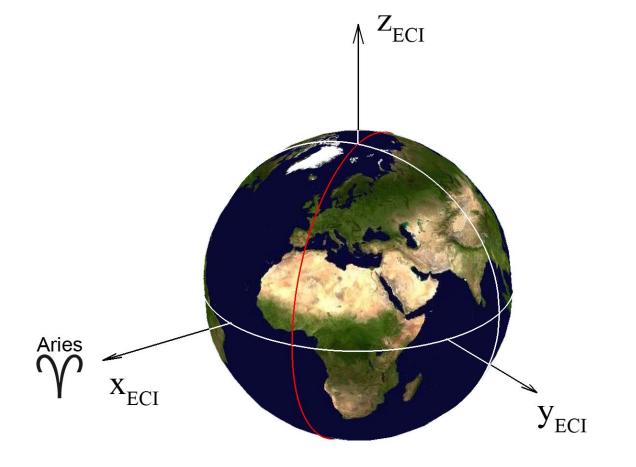
\includegraphics[width=.7\columnwidth]{images/Frame_inercial_terrestre.png}
	\caption{Frame inercial terrestre. Fonte: ~\cite[]{Diaz}}
	\label{fig:Frame_inercial_terrestre}
\end{figure}

\begin{figure}[H]
	\centering
	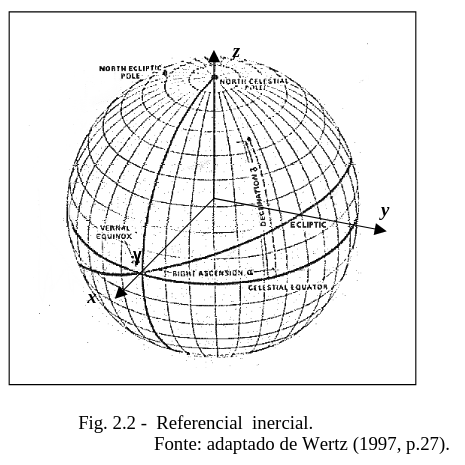
\includegraphics[width=.7\columnwidth, trim=0 60 0 0, clip=true, ]{images/Referencial_inercial.png}
	\caption{Referencial inercial. Fonte: ~\cite[]{Carvalho}}
	\label{fig:Referencial_inercial}
\end{figure}

As estrelas são catalogadas utilizando os pontos de referência, 
utilizando-se de um sistema de coordenadas polares, com duas coordenadas angulares. 
Um dos ângulos é definido a partir dos meridianos, que é a ascensão reta , o ponto de ares é o marco zero, 
a ascensão da reta, que varia de 0 a 360 graus.

A outra coordenada polar é a declinação $\gamma$, que é o ângulo entre a estrela e o paralelo do equador, 
variando de -90 a 90 graus. A Figura ~\ref{fig:Sistema_de_coordenadas_vetorial} mostra sua representação.

\begin{figure}[H]
	\centering
	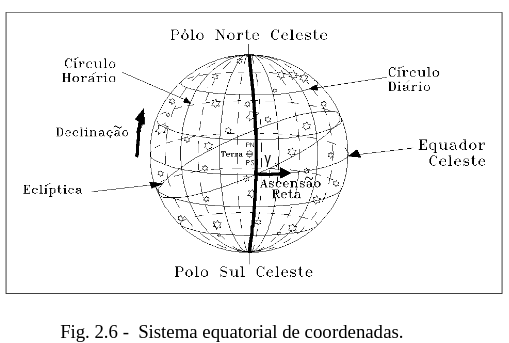
\includegraphics[width=.7\columnwidth, trim={0 30 0 0}, clip]{images/Sistema_equatorial_de_coordenadas.png}
	\caption{Sistema equatorial de coordenadas. Fonte: ~\cite[]{Carvalho}}
	\label{fig:Sistema_equatorial_de_coordenadas}
\end{figure}

A transformação do sistema de coordenadas polares para coordenadas cartesianas é feita  com base na Figura \ref{fig:Sistema_de_coordenadas_vetorial}.

\begin{figure}[H]
	\centering
	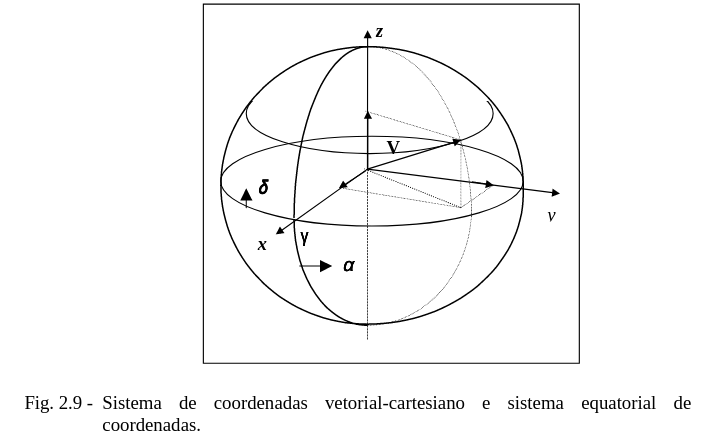
\includegraphics[width=1\columnwidth, trim={0 60 0 0}, clip]{images/Sistema_de_coordenadas_vetorial.png}
	\caption{Sistema de coordenadas vetorial- cartesiano e sistema equatorial de coordenadas. Fonte: ~\cite[]{Carvalho}}
	\label{fig:Sistema_de_coordenadas_vetorial}
\end{figure}

Todas as estrelas catalogadas são descritas na superfície de uma esfera unitária  com centro cociente a Terra, 
portanto, o módulo do vetor que sai do centro da esfera até a estrela é sempre 1,
\begin{equation}
	\left| \overrightarrow{V}\right|=1.
	\label{eq:1}
\end{equation}

Dessa forma, desconsidera-se o valor do raio nas equações de transformação de coordenadas; 
a elaboração das equações é realizada através da análise das relações trigonométricas do sistemas, 
o que resulta em:
\begin{equation}
	V_{x}=cos(\gamma)cos(\alpha),
	\label{eq:2}
\end{equation}

\begin{equation}
	V_{y}=cos(\gamma)sin(\alpha),
	\label{eq:3}
\end{equation}

\begin{equation}
	V_{z}=sin(\gamma).
	\label{eq:4}
\end{equation}

As equação \ref{eq:2}, \ref{eq:3} e \ref{eq:4} são utilizadas para se realizar a decomposição do vetor de coordenadas da estrela, 
está decomposição é feita em relação ao referencial apresentado na Figura \ref{fig:Sistema_de_coordenadas_vetorial}.